\section{Theoretical Analysis}
\label{sec:analysis}

In this section, the circuit shown in Figure~\ref{fig:T2Circuit} is analysed theoretically in six steps.

In step (1), first of all, we used the nodal method to determine the voltages in all nodes and currents in all branches for t<0. The results are shown in Table~\ref{tab:TA1}.

\begin{table}[h]
  \centering
  \begin{tabular}{|l|r|}
    \hline    
    {\bf Nodes and branches} & {\bf Value [V]/[A]} \\ \hline
    v1 & -0.202617 \\ \hline
v2 & -0.619394 \\ \hline
v3 & -5.201027 \\ \hline
v4 & -0.174256 \\ \hline
v5 & 3.485906 \\ \hline
v6 & -7.293091 \\ \hline
v7 & -8.322033 \\ \hline
  \end{tabular}
  \caption{Theoretical voltage values for each node, expressed in Volt, and current values for each branch, expressed in Ampere.}
  \label{tab:TA1}
\end{table}

After this, in step (2), we determined the equivalent resistance as seen from the capacitor terminals. In order to do so, we followed the professor's sugestion: ... The computed results can be found in Table~\ref{tab:TA2}.

\begin{table}[h]
  \centering
  \begin{tabular}{|l|r|}
    \hline    
    {\bf Computed Results} & {\bf Values} \\ \hline
    v1 & -0.202617 \\ \hline
v2 & -0.619394 \\ \hline
v3 & -5.201027 \\ \hline
v4 & -0.174256 \\ \hline
v5 & 3.485906 \\ \hline
v6 & -7.293091 \\ \hline
v7 & -8.322033 \\ \hline
  \end{tabular}
  \caption{Computed results: voltage expressed in Volt, current in Ampere and resistence in Ohm.}
  \label{tab:TA2}
\end{table}

Later, in step (3), we used the value of the equivalent resistant calculated in point (2) to find the natural solution of v6. Knowing that "\tau" is calculated multiplying Req with C(capacitance of the capacitor), in Equation~\ref{eq:natsol} we find the formula required to calculate the natural solution we wanted. 

\begin{equation}
  V_{6n}(t) = V_{x}e^{-\frac{t}{\tau}},
  \label{eq:natsol}
\end{equation}

Also the solution is ploted in Figure~\ref{figure:plotA(4)} where the x-axis corresponds to time, 't', expressed in [ms] and the y-axis corresponds to the natural solution of v6, 'v6n', expressed in [V].

\begin{figure}[h] \centering
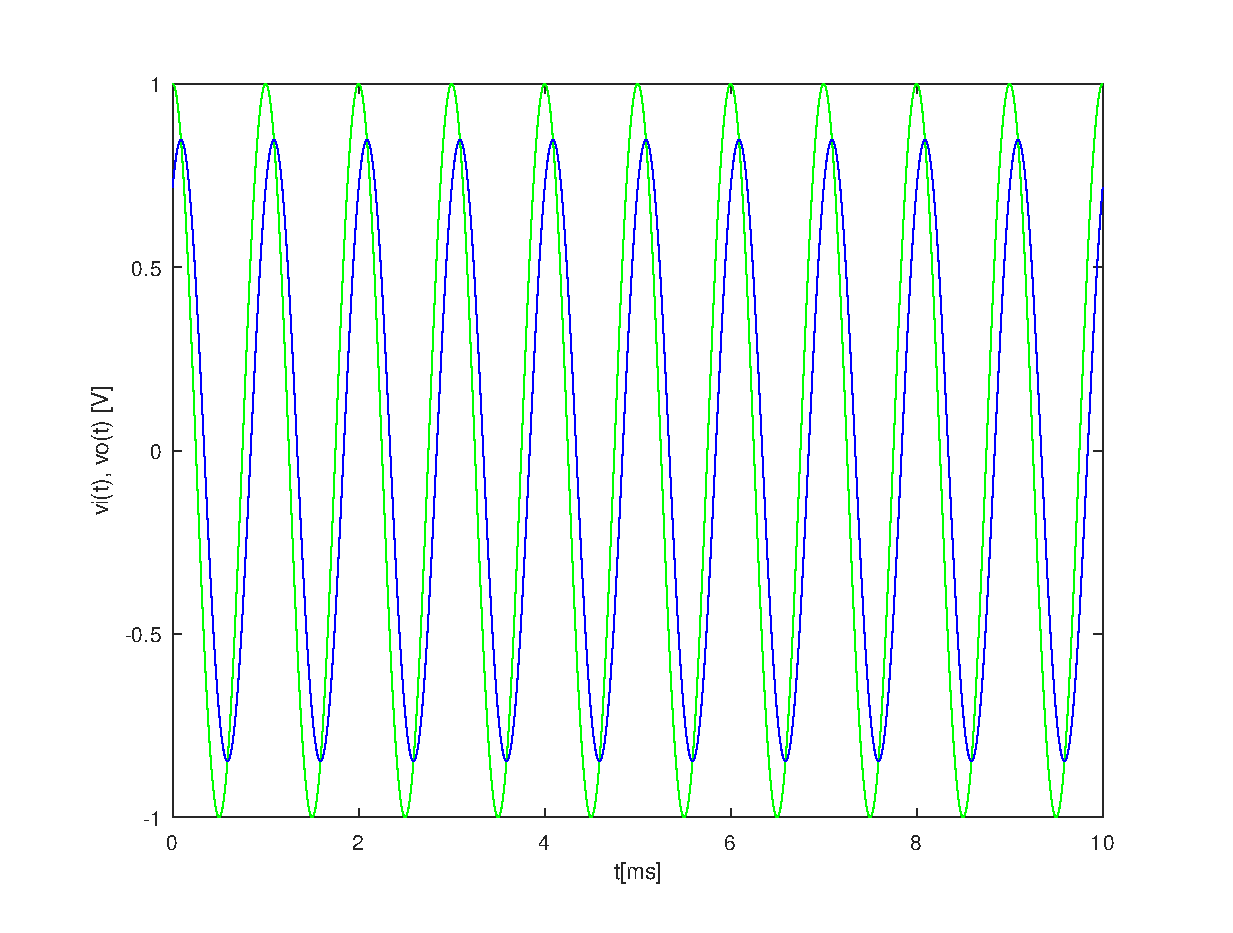
\includegraphics[width=0.8\linewidth]{forced.eps}
\caption{Plot of v6n(t) in the interval [0, 20]ms.}
\label{fig:plotA(4)}
\end{figure}

In step (4), the forced solution v6f(t) was determined for f=1KHz and for 't' in the interval [0,20]ms. Moreover, the capacitance was replaced by the impedance, 'Z', and Vs was considered equal to one. The complex amplitudes in the nodes are shown in Table~\ref{tab:anal4}.

\begin{table}[h]
  \centering
  \begin{tabular}{|l|r|}
    \hline    
    {\bf Nodes} & {\bf Complex Amplitudes} \\ \hline
    \input{op_TAB2}
  \end{tabular}
  \caption{Complex amplitudes in the nodes, expressed in Volt.}
  \label{tab:anal4}
\end{table}













This analysis was performed using the Mesh Method and the Node Method. 
In the Mesh Analysis we used the Kirchoff Voltage Law (KVL) and an additional equation to solve for the currents in the essential meshes. These currents' directions are represented in Figure~\ref{fig:T1Meshes}.

\vspace{6.0cm}

\begin{figure}[h] \centering
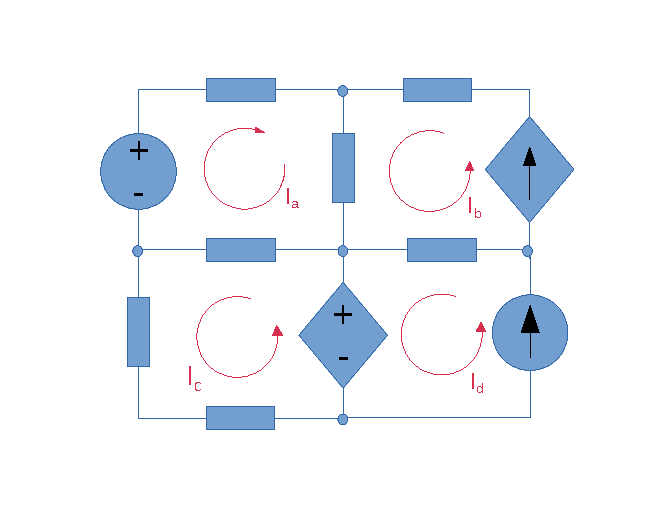
\includegraphics[width=0.4\linewidth]{T1Meshes.pdf}
\caption{Essential meshes' current direction.}
\label{fig:T1Meshes}
\end{figure}

On the other hand, the Node Analysis was done with the Kirchoff Current Law (KCL) applied to the nodes that weren't connected to voltage sources. A supernode was also considered on this analysis in order to simplify the calculation. A supernode was defined by combining the nodes 4 and 7 as these are connected to a voltage source. The supernode equation is found on (5).
The system of equations obtained in each method are presented in the following expressions.

\begin{equation}
  V1(-\frac{1}{R1}-\frac{1}{R2}-\frac{1}{R3}) + V2\frac{1}{R2} + V4\frac{1}{R2} = 0
\end{equation}

\begin{equation}
  V1(Kb+\frac{1}{R2}) -V2\frac{1}{R2} - V4Kb = 0
\end{equation}

\begin{equation}
  V3=-Va
\end{equation}

\begin{equation}
  V1\frac{1}{R3} + V3\frac{1}{R4} + V4(-\frac{1}{R3}-\frac{1}{R4}-\frac{1}{R5}) + V5\frac{1}{R5} + V6\frac{1}{R7} - V7\frac{1}{R7} = Id
\end{equation}

\begin{equation}
  V1Kb - V1(\frac{1}{R5}-Kb) + V5\frac{1}{R5}= Id
\end{equation}

\begin{equation}
  V3\frac{1}{R6} + V5(-\frac{1}{R6}-\frac{1}{R7}) + V7\frac{1}{R7}= 0
\end{equation}

\begin{equation}
  V3\frac{Kc}{R6} - V4 - V6\frac{Kc}{R6} + V7 = 0
\end{equation}

\begin{equation}
  Ia(R1+R2+R3) + IbR3 + IcR4 = Va
\end{equation}

\begin{equation}
  IaR4 + Ic(R4+R6+R7-Kc) = 0
\end{equation}

\begin{equation}
  IaR3 + Ib(-\frac{1}{Kb}+R3) = 0
\end{equation}

\vspace{5.0cm}

After obtaining the system of equations, the Octave tool was used to run all the necessary calculation so as to obtain the theoretical results that are displayed in Table~\ref{tab:nos} and Table~\ref{tab:malhas}.

\begin{table}[h]
  \centering
  \begin{tabular}{|l|r|}
    \hline    
    {\bf Nodes} & {\bf Value [V]} \\ \hline
    v1 & -0.202617 \\ \hline
v2 & -0.619394 \\ \hline
v3 & -5.201027 \\ \hline
v4 & -0.174256 \\ \hline
v5 & 3.485906 \\ \hline
v6 & -7.293091 \\ \hline
v7 & -8.322033 \\ \hline
  \end{tabular}
  \caption{Theoretical voltage values for each node, expressed in Volt.}
  \label{tab:nos}
\end{table}

\begin{table}[h]
  \centering
  \begin{tabular}{|l|r|}
    \hline    
    {\bf Meshes} & {\bf Value [A]} \\ \hline
    Ia & 0.000212 \\ \hline
Ib & -0.000222 \\ \hline
Ic & 0.001098 \\ \hline
  \end{tabular}
  \caption{Theoretical current values for each node, expressed in Ampere.}
  \label{tab:malhas}
\end{table}



